% ============================================================
% Leveraged Purchase — End-to-End Customer Flow
% Trade Republic — Margin Trading Methodology
% Compile with: pdflatex margin_flowchart.tex
% ============================================================

\documentclass[9pt]{article}
\usepackage[a4paper, landscape,
            top=1.0cm, bottom=1.0cm,
            left=1.5cm, right=1.5cm]{geometry}
\usepackage{tikz}
\usetikzlibrary{shapes.geometric, arrows.meta, positioning,
                calc, fit, backgrounds}
\usepackage[T1]{fontenc}
\usepackage[sfdefault]{inter}
\usepackage{amsmath}
\usepackage{microtype}

\pagestyle{empty}
\definecolor{phasegrey}{gray}{0.82}

% ─────────────────────────────────────────────────────────
\begin{document}
% ─────────────────────────────────────────────────────────

\begin{center}
  {\large\bfseries Leveraged Purchase — Customer End-to-End Flow}\\[2pt]
  {\scriptsize\itshape
    Trade Republic Margin Requirements Methodology — Sections D \& E
    \hfill \textsc{Strictly Private \& Confidential}}
\end{center}
\vspace{2pt}

\centering
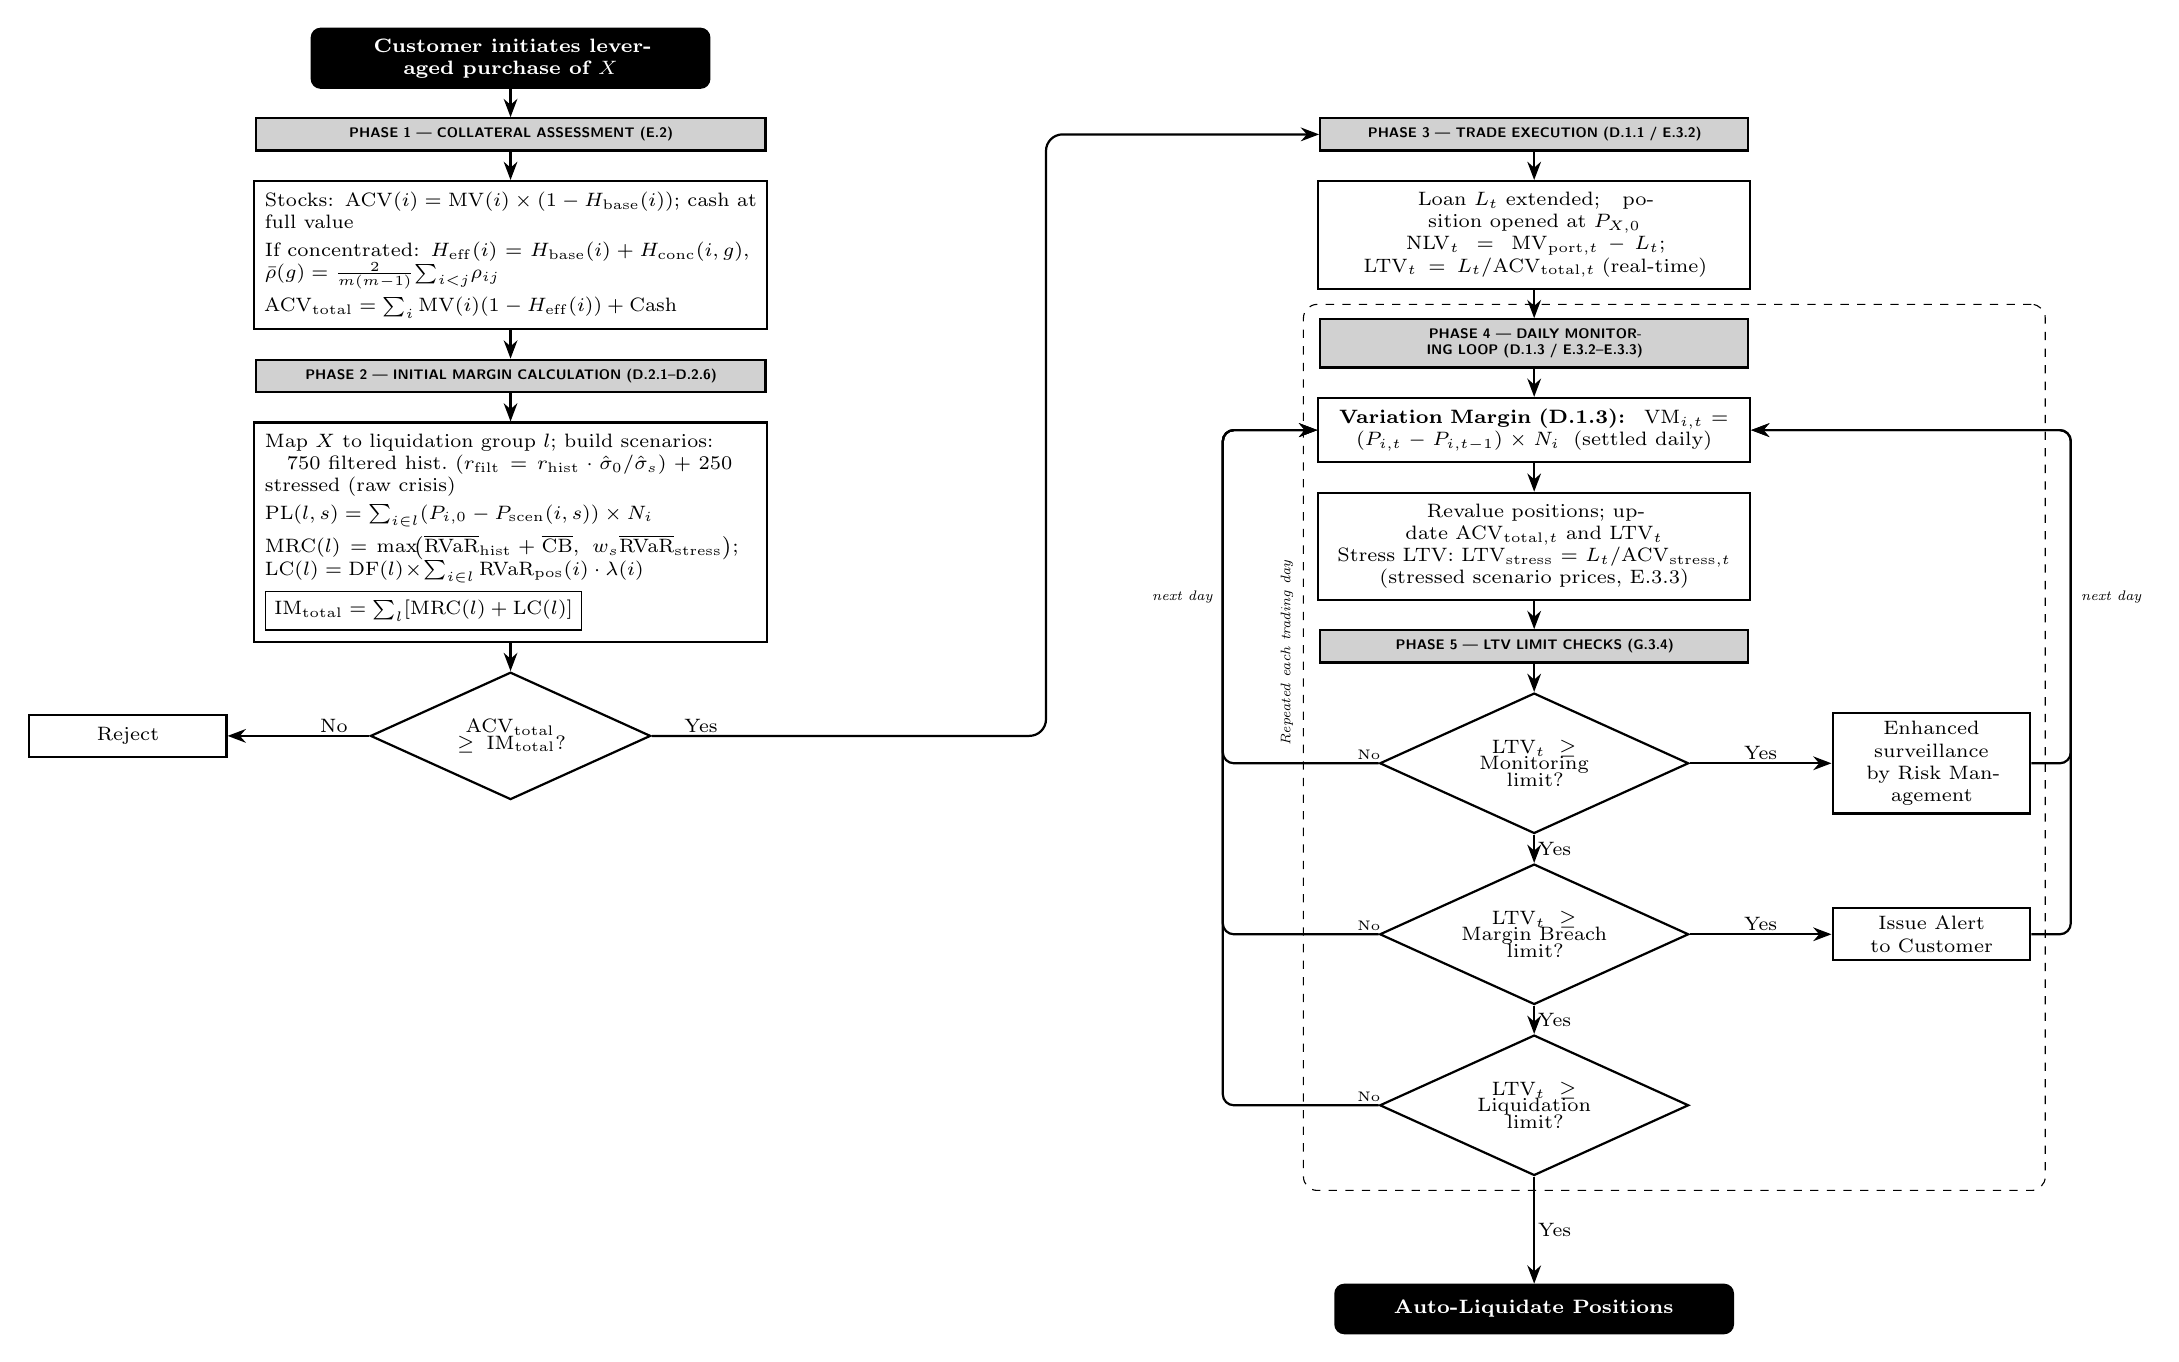
\begin{tikzpicture}[
  node distance = 0.36cm and 1.8cm,
  proc/.style  = {rectangle, draw=black, thick,
                  text width=5.2cm, minimum height=0.62cm,
                  align=center, font=\scriptsize, inner sep=4pt},
  procl/.style = {rectangle, draw=black, thick,
                  text width=5.2cm, align=left,
                  font=\scriptsize, inner sep=4pt},
  % left-column variants — 20% wider (5.2 × 1.2 = 6.24 cm)
  procll/.style = {rectangle, draw=black, thick,
                   text width=6.24cm, align=left,
                   font=\scriptsize, inner sep=4pt},
  pbarl/.style  = {rectangle, draw=black, thick, fill=phasegrey,
                   text width=6.24cm, minimum height=0.38cm,
                   align=center, font=\tiny\bfseries\sffamily},
  dec/.style   = {diamond, draw=black, thick,
                  text width=2.4cm, minimum height=0.70cm,
                  align=center, font=\scriptsize, aspect=2.2, inner sep=1pt},
  term/.style  = {rectangle, rounded corners=3pt,
                  draw=black, very thick, fill=black, text=white,
                  text width=4.8cm, minimum height=0.60cm,
                  align=center, font=\scriptsize\bfseries},
  pbar/.style  = {rectangle, draw=black, thick, fill=phasegrey,
                  text width=5.2cm, minimum height=0.38cm,
                  align=center, font=\tiny\bfseries\sffamily},
  side/.style  = {rectangle, draw=black, thick,
                  text width=2.3cm, minimum height=0.54cm,
                  align=center, font=\scriptsize, inner sep=3pt},
  arr/.style   = {-Stealth, thick},
  lbl/.style   = {font=\scriptsize, inner sep=1pt},
]

%% ══════════════════════════════════════════════════════════
%%  LEFT COLUMN — Phases 1 & 2  (centre x = −6.5 cm)
%% ══════════════════════════════════════════════════════════

\node[term] at (-6.5, 0) (start)
  {Customer initiates leveraged purchase of~$X$};

\node[pbarl, below=of start] (pbar1)
  {PHASE 1 — COLLATERAL ASSESSMENT (E.2)};

\node[procll, below=of pbar1] (coll)
  {Stocks: $\mathrm{ACV}(i)=\mathrm{MV}(i)\times(1-H_{\rm base}(i))$;
   cash at full value\\[2pt]
   If concentrated: $H_{\rm eff}(i)=H_{\rm base}(i)+H_{\rm conc}(i,g)$,
   \;$\bar\rho(g)=\tfrac{2}{m(m-1)}\!\sum_{i<j}\!\rho_{ij}$\\[2pt]
   $\mathrm{ACV}_{\rm total}
     =\textstyle\sum_i\mathrm{MV}(i)(1-H_{\rm eff}(i))+\mathrm{Cash}$};

\node[pbarl, below=of coll] (pbar2)
  {PHASE 2 — INITIAL MARGIN CALCULATION (D.2.1–D.2.6)};

\node[procll, below=of pbar2] (imCalc)
  {Map $X$ to liquidation group $l$; build scenarios:\\
   \quad 750 filtered hist.\ ($r_{\rm filt}=r_{\rm hist}\cdot\hat\sigma_0/\hat\sigma_s$)
   + 250 stressed (raw crisis)\\[2pt]
   $\mathrm{PL}(l,s)=\sum_{i\in l}(P_{i,0}-P_{\rm scen}(i,s))\times N_i$\\[2pt]
   $\mathrm{MRC}(l)=\max\!\bigl(
     \overline{\rm RVaR}_{\rm hist}+\overline{\rm CB},\;
     w_s\overline{\rm RVaR}_{\rm stress}\bigr)$;\quad
   $\mathrm{LC}(l)=\mathrm{DF}(l)\!\times\!
     \textstyle\sum_{i\in l}\mathrm{RVaR}_{\rm pos}(i)\cdot\lambda(i)$\\[2pt]
   \centering
   $\boxed{\mathrm{IM}_{\rm total}
     =\textstyle\sum_l[\mathrm{MRC}(l)+\mathrm{LC}(l)]}$};

\node[dec, below=of imCalc] (colChk)
  {$\mathrm{ACV}_{\rm total}$\\[-2pt]$\geq\mathrm{IM}_{\rm total}$?};

\node[side, left=of colChk] (reject)
  {Reject};

%% ══════════════════════════════════════════════════════════
%%  RIGHT COLUMN — Phases 3–5  (centre x = +6.5 cm)
%%  Anchored at same y as pbar1 so both columns are level.
%% ══════════════════════════════════════════════════════════

\node[pbar] at ($(pbar1) + (13, 0)$) (pbar3)
  {PHASE 3 — TRADE EXECUTION (D.1.1 / E.3.2)};

\node[proc, below=of pbar3] (openPos)
  {Loan $L_t$ extended;\quad position opened at $P_{X,0}$\\
   $\mathrm{NLV}_t=\mathrm{MV}_{{\rm port},t}-L_t$;\quad
   $\mathrm{LTV}_t=L_t/\mathrm{ACV}_{{\rm total},t}$\;(real-time)};

\node[pbar, below=of openPos] (pbar4)
  {PHASE 4 — DAILY MONITORING LOOP (D.1.3 / E.3.2–E.3.3)};

\node[proc, below=of pbar4] (vm)
  {\textbf{Variation Margin (D.1.3):}
   $\;\mathrm{VM}_{i,t}=(P_{i,t}-P_{i,t-1})\times N_i$\; (settled daily)};

\node[proc, below=of vm] (revalue)
  {Revalue positions; update $\mathrm{ACV}_{{\rm total},t}$ and $\mathrm{LTV}_t$\\
   Stress~LTV: $\mathrm{LTV}_{\rm stress}=L_t/\mathrm{ACV}_{{\rm stress},t}$
   (stressed scenario prices, E.3.3)};

\node[pbar, below=of revalue] (pbar5)
  {PHASE 5 — LTV LIMIT CHECKS (G.3.4)};

\node[dec, below=of pbar5] (monChk)
  {$\mathrm{LTV}_t\geq$\\[-2pt]Monitoring\\[-2pt]limit?};

\node[dec, below=of monChk] (breachChk)
  {$\mathrm{LTV}_t\geq$\\[-2pt]Margin Breach\\[-2pt]limit?};

\node[dec, below=of breachChk] (liqChk)
  {$\mathrm{LTV}_t\geq$\\[-2pt]Liquidation\\[-2pt]limit?};

\node[term, below=of liqChk, yshift=-1cm] (autoLiq)
  {Auto-Liquidate Positions};

%% ── Right-side action boxes ───────────────────────────────

\node[side, right=of monChk]    (flag)
  {Enhanced surveillance\\by Risk Management};

\node[side, right=of breachChk] (mcall)
  {Issue Alert\\ to Customer};

%% ══════════════════════════════════════════════════════════
%%  ARROWS — LEFT COLUMN
%% ══════════════════════════════════════════════════════════

\draw[arr] (start)   -- (pbar1);
\draw[arr] (pbar1)   -- (coll);
\draw[arr] (coll)    -- (pbar2);
\draw[arr] (pbar2)   -- (imCalc);
\draw[arr] (imCalc)  -- (colChk);
\draw[arr] (colChk)  -- node[lbl, above, near start]{No} (reject);

%% ══════════════════════════════════════════════════════════
%%  CONNECTING ARROW: "Yes" from colChk → Phase 3
%%  Routes through the inter-column space (around x = +0.3)
%%  to avoid crossing the hconc→acvT path in the left column.
%% ══════════════════════════════════════════════════════════

% Inter-column waypoint x-coordinate (between the two columns)
\coordinate (icx) at (0.3, 0);

\draw[arr, rounded corners=6pt]
  (colChk.east)
  -- node[lbl, above, very near start]{Yes}
  (icx |- colChk.east)    % same y as colChk, x = 0.3
  -- (icx |- pbar3.west)  % same y as pbar3, x = 0.3
  -- (pbar3.west);         % enter right column

%% ══════════════════════════════════════════════════════════
%%  ARROWS — RIGHT COLUMN
%% ══════════════════════════════════════════════════════════

\draw[arr] (pbar3)      -- (openPos);
\draw[arr] (openPos)    -- (pbar4);
\draw[arr] (pbar4)      -- (vm);
\draw[arr] (vm)         -- (revalue);
\draw[arr] (revalue)    -- (pbar5);
\draw[arr] (pbar5)      -- (monChk);
\draw[arr] (monChk)     -- node[lbl, right]{Yes} (breachChk);
\draw[arr] (breachChk)  -- node[lbl, right]{Yes} (liqChk);
\draw[arr] (liqChk)     -- node[lbl, right]{Yes} (autoLiq);

\draw[arr] (monChk)    -- node[lbl, above]{Yes} (flag);
\draw[arr] (breachChk) -- node[lbl, above]{Yes}      (mcall);

%% ══════════════════════════════════════════════════════════
%%  LOOP-BACK ARROWS — "next trading day"
%%  All route via a left rail inside the right column.
%% ══════════════════════════════════════════════════════════

% Left loop rail: just left of the right column
\coordinate (LLR) at ($(vm.west) + (-1.2, 0)$);

% Shared right rail: 0.5 cm past the right edge of the flag/mcall boxes,
% ensuring both "next day" arrows travel the same vertical path to vm.
\coordinate (RLR) at ($(flag.east) + (0.5, 0)$);

% "No" from monChk → next day
\draw[arr, rounded corners=4pt]
  (monChk.west) -- node[lbl, above]{\tiny No} ++(-0.25,0)
  -- (LLR |- monChk.west)
  -- node[pos=0.5, left, font=\tiny\itshape]{next day}
     (LLR |- vm.west)
  -- (vm.west);

% "No" from breachChk → next day (same rail)
\draw[arr, rounded corners=4pt]
  (breachChk.west) -- node[lbl, above]{\tiny No} ++(-0.25,0)
  -- (LLR |- breachChk.west)
  -- (LLR |- vm.west)
  -- (vm.west);

% "No" from liqChk → next day (same rail)
\draw[arr, rounded corners=4pt]
  (liqChk.west) -- node[lbl, above]{\tiny No} ++(-0.25,0)
  -- (LLR |- liqChk.west)
  -- (LLR |- vm.west)
  -- (vm.west);

% flag → next day (shared right rail)
\draw[arr, rounded corners=4pt]
  (flag.east)
  -- (RLR |- flag.east)
  -- node[pos=0.5, right, font=\tiny\itshape]{next day}
     (RLR |- vm.east)
  -- (vm.east);

% mcall → next day (same shared right rail)
\draw[arr, rounded corners=4pt]
  (mcall.east)
  -- (RLR |- mcall.east)
  -- (RLR |- vm.east)
  -- (vm.east);

%% ══════════════════════════════════════════════════════════
%%  DASHED BOX — daily monitoring loop highlight
%% ══════════════════════════════════════════════════════════

\begin{pgfonlayer}{background}
  \node[draw=black, thin, dashed, rounded corners=5pt, inner sep=5pt,
        fit=(pbar4)(vm)(revalue)(pbar5)(monChk)(breachChk)(liqChk)
            (flag)(mcall)] (loopBox) {};
\end{pgfonlayer}

\node[font=\tiny\itshape, rotate=90, anchor=south]
  at ($(loopBox.west) + (0, 1.2cm)$) {Repeated each trading day};

\end{tikzpicture}

\vspace{4pt}
\end{document}
